\documentclass[xcolor=dvipsnames]{beamer}
%\usepackage{beamerthemelined}
\usepackage{amsfonts,amssymb,amsmath}
\usepackage{mathtools}
\usepackage{graphicx}
\usepackage{color}

\setbeamertemplate{caption}{\insertcaption} % remove the word 'figure' before captions

\usetheme{Frankfurt}
%% \useinnertheme{rounded}
%% \useoutertheme{infolines}
\usecolortheme{dolphin}
\usecolortheme[named=OliveGreen]{structure}
\beamertemplatenavigationsymbolsempty
%% \setbeamertemplate{footline}[page number]

%% Citations
\newcommand{\myciteetal}[3]{{\tiny #1 \emph{et al}, \textit{#2} (#3)}}
\newcommand{\mycite}[3]{{\tiny #1, \textit{#2} (#3)}}

%% n values
\newcommand{\npart}{\ensuremath{n_{part}}}
\newcommand{\nvap}{\ensuremath{n_{vap}}}
\newcommand{\nliq}{\ensuremath{n_{liq}}}

%% 1/kT
\newcommand{\kT}{\ensuremath{k_{B}T}}

%% Lambda values
\newcommand{\lambdaSW}{\ensuremath{\lambda_\text{sw}}}
\newcommand{\lambdaRG}{\ensuremath{\lambda_\text{rg}}}

%% Free energy
\newcommand{\Fex}{\ensuremath{F_\text{ex}}}

%% Vectors
\newcommand{\rr}{\ensuremath{\mathbf{r}}}
\newcommand{\pp}{\ensuremath{\mathbf{p}}}

% TPT
\newcommand{\III}{\ensuremath{\textbf{r}_{12}}} % Roman numerals for \12
\newcommand{\Vtilde}{\ensuremath{\widetilde{V}}}
\newcommand{\Wtilde}{\ensuremath{\widetilde{W}}}

%% fixme
\newcommand{\fixme}[1]{\textcolor{red}{\textbf{[#1]}}}

%-----------------------------------------
% TITLE
%-----------------------------------------

\title[Applying RGT to SW liquid]{Applying Renormalization Group Theory to the Square Well Liquid}
\author[Roth \& Roundy]{Dan Roth}
\institute[OSU]{Oregon State University}
\date{12 June 2014}

\begin{document}


\begin{frame}
  \titlepage
\end{frame}

%-----------------------------------------
% TOC
%-----------------------------------------
\section{}
\begin{frame}{Overview}
  \tableofcontents
\end{frame}

%-----------------------------------------
% INTRO
%-----------------------------------------
\section{Introduction}

\subsection{} %% Liquid
\begin{frame}{What is a liquid?}
  \framesubtitle{Simple definition}
  \begin{block}{Liquid}
    Something that takes the shape of its container, but does not necessarily fill the container
  \end{block}
  \begin{itemize}
    \item Pretty good, but a bit too simple $\rightarrow$ some things could be classified as a liquid that should not be
  \end{itemize}
  \onslide<2->{
    \begin{center}
      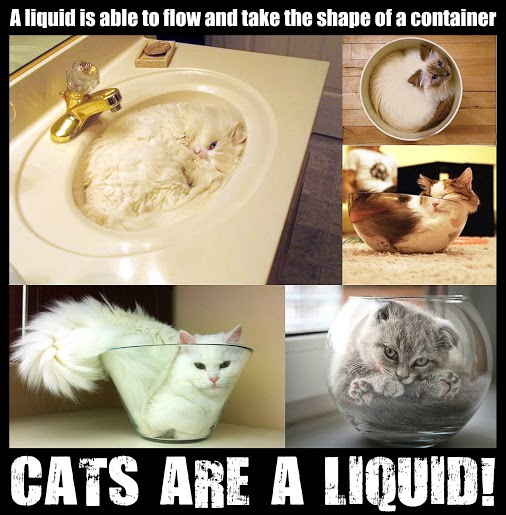
\includegraphics[width=0.4\textwidth]{figs/cat-liquid-2} \\
%%      \tiny{\url{http://newauthorpublishing.wordpress.com/2013/08/06/895}}
    \end{center}
    }
\end{frame}

\begin{frame}{What is a liquid?}
  \framesubtitle{More advanced definition}
  \begin{block}{Liquid}
    Phase of matter where neither energy nor entropy are dominant
  \end{block}

  We use perturbation theory to investigate liquids:
  \begin{itemize}
    \item Take an ``easy'' problem we know how to solve
    \item Add a ``difficult'' correction that is small
    \item Construct a power series to solve combined problem
  \end{itemize}
\end{frame}

\begin{frame}{Hard Spheres}
  For the ``easily'' solved problem we use a \emph{hard sphere liquid}:
  \begin{itemize}
    \item Not actually easy to solve $\rightarrow$ never been solved exactly, but good approximations have been made
    \item Spheres cannot overlap (they are ``hard'')
    \item No attraction between spheres
      \begin{itemize}
        \item<1->Simulations are simple
        \item<2->Not actually a liquid
      \end{itemize}
  \end{itemize}
  \begin{center}
    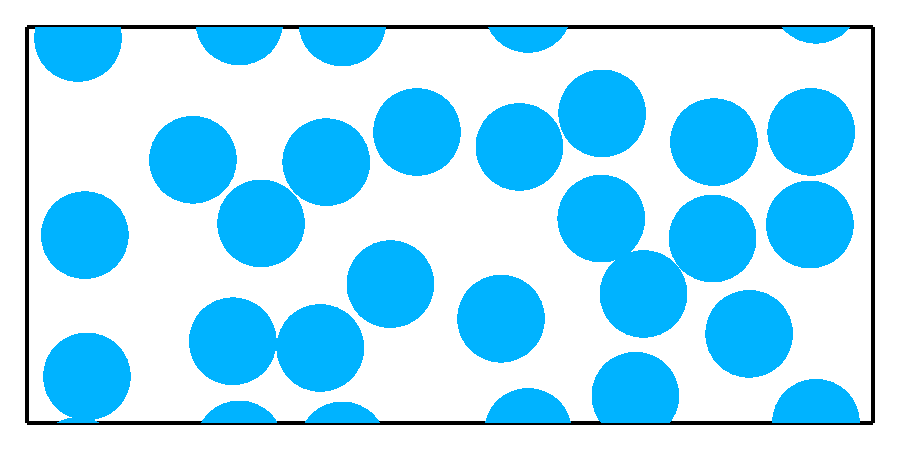
\includegraphics[width=0.75\textwidth]{figs/hard-spheres}
  \end{center}
\end{frame}

\begin{frame}{Square well attraction}
  Attraction is what makes this system a liquid
  \begin{columns}
    \column{0.5\textwidth}
    \begin{itemize}
      \item Each molecule is a sphere with diameter $\sigma$
      \item Infinite potential when two spheres are touching
      \item Constant attractive potential $-\varepsilon$ for some distance $\lambdaSW\sigma$
      \item Zero potential to infinity (and beyond)
    \end{itemize}

    \column{0.6\textwidth}
    \begin{center}
      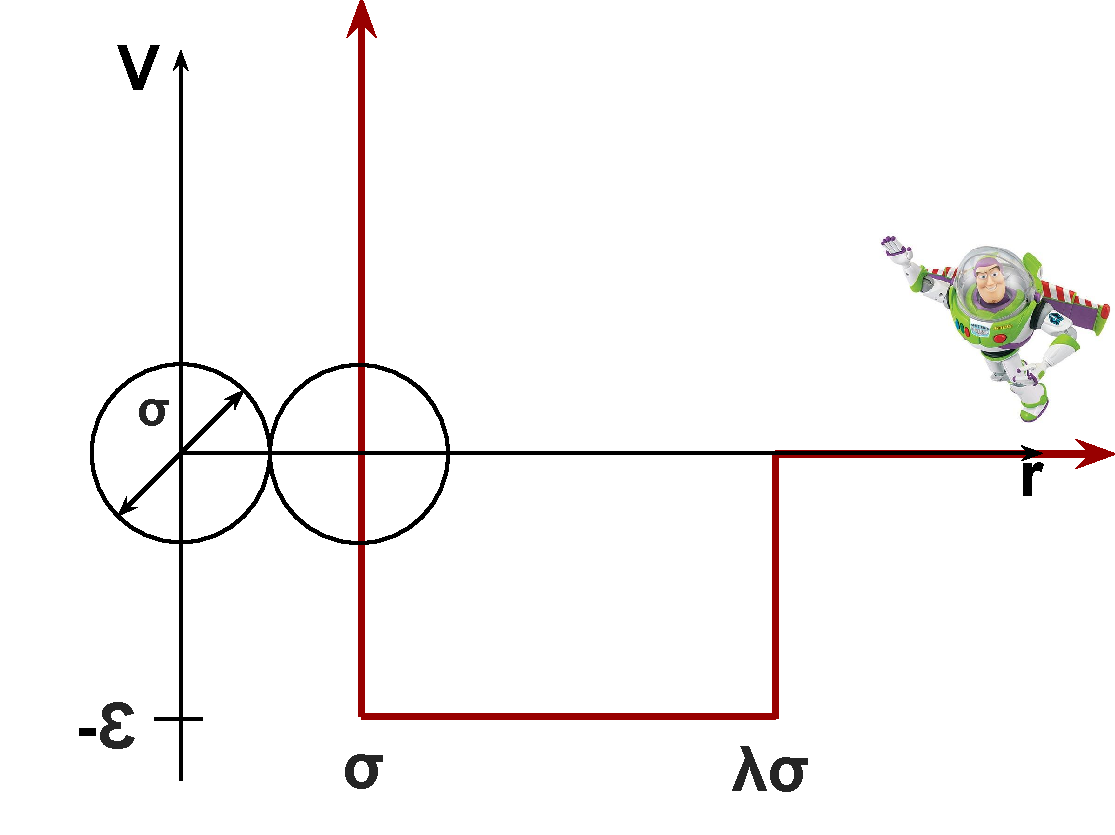
\includegraphics[width=\columnwidth]{figs/SW-schematic-buzz}
    \end{center}
  \end{columns}
%%   There seem to be infinite forces at the boundaries, but forces play no role in thermodynamic averages
\end{frame}

\subsection{} %% Some basic Stat Mech.
\begin{frame}{Statistical Mechanics Basics}
  \begin{block}{Partition Function}
    \begin{itemize}
      \item Sum up the \emph{Boltzmann factor} of every possible microstate of the system
    \end{itemize}
     \[ Z = \sum_i^\text{\tiny{microstates}}e^{-\beta E_i} \quad\quad  \beta \equiv \frac{1}{\kT} \]
  \end{block}

  We can also write this as an integral:
  \begin{align*}
    Z &= \frac{1}{h^{3N}N!}\int d\rr^N d\pp^N\, \exp\left( -\frac{\beta}{2m}\sum p^2 - \beta U(r) \right) \\
    &= \frac{1}{h^{3N}N!}\int d\pp^N\, \exp\left( -\frac{\beta}{2m}\sum p^2 \right)\int d\rr^N\, \exp(-\beta U(r)) \\
    &= Z_\text{id}Z_\text{ex}
  \end{align*}

\end{frame}

\begin{frame}{Statistical Mechanics Basics}
  \begin{block}{Helmholtz free energy}
    \begin{itemize}
      \item Know Helmholtz $\rightarrow$ figure out anything else you want to know
      \item Useful for fixed temperature and particle number
    \end{itemize}
    \[ F = U - TS = -k_BT\ln Z \]
  \end{block}

  \begin{block}{Grand free energy}
    \begin{itemize}
      \item Number of particles not fixed
      \item Calculate from Helmholtz
    \end{itemize}
    \[ \varPhi = F - N\mu \]
  \end{block}

  \begin{block}{Chemical potential $\mu$}
    Energy cost that the environment must pay to add a particle to the system
  \end{block}
\end{frame}

\subsection{} %% Critical point

\begin{frame}{Critical Point}
  \begin{center}
    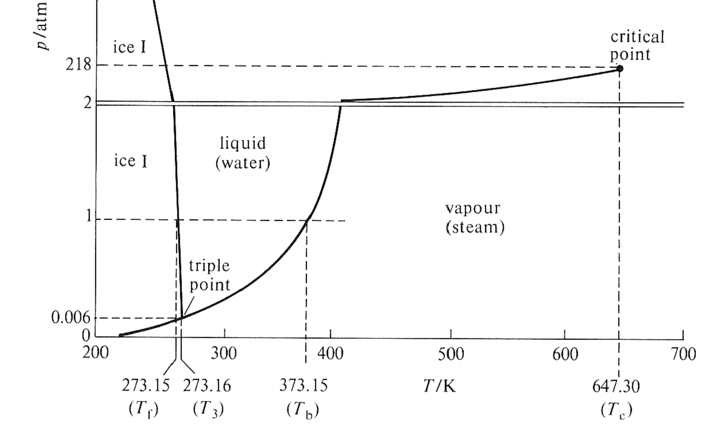
\includegraphics[width=0.7\textwidth]{figs/phase-diagram-zoom}

    Phase diagram for water
  \end{center}

  \begin{itemize}
    \item Lines are where two phases can exist in equilibrium
  \end{itemize}

\end{frame}

\begin{frame}{Density fluctuations}
  \begin{columns}[T]
  \column{0.6\textwidth}
  \includegraphics<1>[width=\columnwidth]{~/deft/papers/renormalization/figs/fluctuations}
  \includegraphics<2>[width=\columnwidth]{figs/critical-opalescence}

  \onslide<2>{Size of fluctuations comparable with wavelength of light near the critical point}

  \column{0.4\textwidth}
  \begin{itemize}
    \item Take a snapshot in time
    \item At the critical point, there are fluctuations in density at all length scales
    \item Makes perturbation theories fall apart
    \item Visible effect: critical opalescence
  \end{itemize}
  \end{columns}
\end{frame}

\subsection{} %% Motivation for this work
\begin{frame}{Motivation}
  \begin{block}{Importance of critical point}
  \begin{itemize}
  \item Supercritical fluids used in many industrial processes, such as
    \begin{itemize}
    \item Extraction of caffeine from coffee beans \\ (very relevant in PNW)
    \item Extraction of hops resins for beer production \\ (also relevant in PNW)
    \item Decomposing biomass for hydrocarbon fuel production
    \item \ldots and many more
    \end{itemize}
  \end{itemize}
  \end{block}

  \begin{itemize}
    \item Using TPT and RGT should give us a good way of studying the critical point of a liquid
    \item We start with the square well liquid because it is a widely-used approximation to simple liquids
    \item We want to see if implementing RGT would be worthwhile to this research group
    \begin{itemize}
      \item Other groups use RGT, but don't mention computational cost
    \end{itemize}
  \end{itemize}
\end{frame}

%-----------------------------------------
% TPT
%-----------------------------------------
\section[TPT]{Thermodynamic Perturbation Theory}
\subsection{}

\begin{frame}{Quantum Perturbation Theory}
  \begin{block}{Hamiltonian}
    Sum of kinetic and potential energy terms
  \end{block}
  \begin{enumerate}
    \item Start with a Hamiltonian we can solve analytically, $\widetilde{H}_0$
    \item Add a small change, $\xi \Wtilde$
    \item The complete Hamiltonian of the system is then: $ \widetilde{H} = \widetilde{H}_0 + \xi \Wtilde $
    \item Apply to the Schroedinger equation: $ \widetilde{H}|n\rangle = E|n\rangle \Rrightarrow (\widetilde{H}_0 + \xi \Wtilde)|n\rangle = E|n\rangle $
    \item For small values of $\xi$, we can expand $E$ and $|n\rangle$ as power series: \[ E_n = E_n^{(0)} + \xi E_n^{(1)} + \xi^2E_n^{(2)} + \cdots \] and \[ |n\rangle = |n^{(0)}\rangle + \xi|n^{(1)}\rangle + \xi^2|n^{(2)}\rangle + \cdots \]
  \end{enumerate}
\end{frame}

\begin{frame}{Thermodynamic Perturbation Theory}
  \begin{itemize}
    \item For TPT we are perturbing the potential only, not the entire Hamiltonian
  \end{itemize}

  \begin{block}{The reference system}
    \begin{itemize}
      \item Hard sphere potential
    \end{itemize}
    \[
      v_\text{hs}(\III) =
      \begin{cases}
        \infty & r \leq \sigma \\
        0 & \sigma < r
      \end{cases}
    \]
  \end{block}

  \begin{block}{Perturbation}
    \begin{itemize}
      \item Square well attraction
    \end{itemize}
    \[
      w_\text{sw}(\III) = - \varepsilon \quad  \sigma < r < \lambdaSW\sigma
    \]
  \end{block}

  \begin{block}{}
  \[ v(\III) = v_\text{hs}(\III) + w_\text{sw}(\III) \]
  \end{block}
\end{frame}

\begin{frame}{Excess Free Energy}
  The total potential energy of our system is \[ \Vtilde = \sum_{i=1}^N\sum_{j>i}^N \left( v_\text{hs}(\rr_{ij}) + \xi w_\text{sw}(\rr_{ij}) \right) \]
  The \emph{configuration integral} is the potential energy component of the partition function: \[ Z_\xi = \frac{1}{V^N}\int d\rr^N\, e^{-\beta \Vtilde} \] where volume to the $N^{th}$ power has shown up for normalization.
  From the configuration integral we can get the excess (from ideal) free energy:\[ \Fex = -\kT\ln Z_\xi \]
  \mycite{Hansen \& McDonald}{Academic Press}{2006}
\end{frame}

\begin{frame}{Derivative}
  It is easier, and no less exact, to work with the derivative of \Fex:
    \begin{align*}
    \frac{\partial \Fex}{\partial\xi} &=-\kT\frac{\partial}{\partial\xi}\left( \ln Z_\xi \right)  \\
    &\vdots \\
    &= \frac{1}{Z_\xi} \int d\rr^N\, \Wtilde e^{-\beta \Vtilde} \\
    &= \left\langle \Wtilde \right\rangle_{\xi}
  \end{align*}
  where $\Wtilde = \partial \Vtilde/\partial \xi$ and $\left\langle \Wtilde\right\rangle_{\xi}$ is the ensemble average of $\Wtilde$ for some value of $\xi$
\end{frame}


\begin{frame}{Expansion}
  Now take a series expansion of $\left\langle W_N\right\rangle_{\xi}$ around $\xi = 0$
  \begin{align*}
    \left\langle \Wtilde \right\rangle_{\xi} &= \left\langle \Wtilde\right\rangle_{\xi = 0} + (\xi)\frac{\partial\left\langle \Wtilde \right\rangle_{\xi}}{\partial\xi}\bigg|_{\xi = 0} + \mathcal{O}(\xi^2)
  \end{align*}
  And the derivative term is
  \begin{align*}
    \frac{\partial}{\partial\xi}\left\langle \Wtilde \right\rangle_{\xi} &= \frac{\partial}{\partial\xi}\left( \frac{1}{Z_\xi}\int d\rr^N\, \Wtilde e^{-\beta \Vtilde}\right)  \\
    &\vdots  \\
    &= -\beta\left[ \left\langle \Wtilde^2 \right\rangle_{\xi} - \left\langle \Wtilde \right\rangle_{\xi}^2 \right]  \\
    &\equiv -\beta\sigma_{\xi}^2 \quad \text{Note that $\sigma^2 > 0 \rightarrow$ this term is always negative}
  \end{align*}
  So we have
  \begin{align*}
    \left\langle \Wtilde \right\rangle_{\xi} &= \left\langle \Wtilde\right\rangle_{\xi = 0} - (\xi)\beta\sigma_{\xi=0}^2 + \mathcal{O}(\xi^2)
  \end{align*}
\end{frame}

%% \begin{frame}{Integrate to get \emph{High Temperature Expansion}}
%%   Limits of integration:
%%   \begin{itemize}
%%     \item $ F \in [F_\text{ref},\Fex] $
%%     \item $ \xi \in [0,1] $
%%   \end{itemize}
%%   \begin{align*}
%%     \Fex - F_\text{ref} &= (1-0)\left\langle \Wtilde \right\rangle_{\xi=0} - \frac{1}{2}\beta(1 - 0)^2\sigma_{\xi=0}^2 + \mathcal{O}(\beta^2)  \\
%%     \hookrightarrow \Fex &= F_\text{ref} + \left\langle \Wtilde \right\rangle_{\xi=0} - \frac{1}{2}\beta\sigma_{\xi=0}^2 + \mathcal{O}(\beta^2) \\
%%   \end{align*}
%%   \mycite{Robert Zwanzig}{J.~Chem.~Phys.}{1954}
%% \end{frame}

\begin{frame}{High Temperature Expansion}
  Integrate to get back to the free energy
  \begin{align*}
    \Fex &= F_\text{ref} + \left\langle \Wtilde \right\rangle_{\xi=0} - \frac{1}{2}\beta\sigma_{\xi=0}^2 + \mathcal{O}(\beta^2) \\
    \Fex &= F_\text{ref} + A_1(n) + \beta A_2(n) + \mathcal{O}(\beta^2)
  \end{align*}
  with
  \begin{align*}
    A_1(n) &= \frac{1}{Z_\xi}\int d\rr^N\, \Wtilde e^{-\beta\Vtilde} \qquad A_2(n) = -\frac{\sigma_{\xi=0}^2}{2}
  \end{align*}
  \begin{itemize}
    \item $A_1$ is the ``zeroth'' order interaction between molecules
    \item $A_2$ is a bit more complicated; to exactly determine it, we need to know higher-order correlations
    \item We approximate $A_2$ with the local compressibility approximation
  \end{itemize}
  \mycite{Robert Zwanzig}{J.~Chem.~Phys.}{1954}
\end{frame}

%-----------------------------------------
% RGT
%-----------------------------------------
\section[RGT]{Renormalization Group Theory}
\subsection{}

\begin{frame}{Account for fluctuations at all length scales}
  \begin{block}{Basic idea behind TPT}
    Take a baseline and consider small changes in the attractive potential
  \end{block}

  \begin{block}{Basic idea behind RGT}
    Take a baseline and consider not-so-small changes in the free energy
  \end{block}

  RGT is an iterative procedure:
  \begin{itemize}
    \item Start with a baseline free energy---we use thermodynamic perturbation theory (TPT)
    \item Add corrections
  \end{itemize}

  \begin{block}{Historical note}
    Developed in the 1950s; work by Kenneth Wilson in the '70s won him the 1982 Nobel Prize in physics
  \end{block}
\end{frame}

\begin{frame}{Renormalization Group Theory}
  \begin{itemize}
    \item Consider density fluctuations\ldots
    \item Fluctuations of wavelength $\lambdaRG < \lambda_0$ are assumed to be accounted for in the baseline free energy (TPT for this work)
    \item What if we include fluctuations of wavelength $2\lambda_0$? How about $4\lambda_0$? \ldots and so on
    \item Divide up all space into cells; each cell has a volume \[V_\text{cell,i} = \left(\frac{2^i\lambda_0}{2}\right)^3\] where $i$ is the iteration you are on and $\lambda_0$ is the cutoff wavelength
    \item Within a cell, we assume that the density is only slowly varying
  \end{itemize}
\end{frame}

\begin{frame}{Iterations}
  \begin{align*}
    F_1 &= F_0 + \delta F_0  \\
    F_2 &= F_1 + \delta F_1  \\
%%     F_3 &= F_2 + \delta F_2  \\
    &\vdots  \\
    F_i(T,n) &= F_{i-1}(T,n) + \delta F_{i-1}(T,n) \\
    \hookrightarrow F &= F_0 + \sum_i\delta F_i(T,n) \\
    \delta F_i(T,n) &= -k_BT\ln\left( \frac{Z_i}{Z_i^*} \right)
  \end{align*}

  \begin{itemize}
    \item The ratio in the log is nothing more than a free energy difference
    \item $Z_i$ is the partition function for the entire system
    \item $Z_i^*$ is the partition function of a reference system that does not contain fluctuations
  \end{itemize}
\end{frame}

\begin{frame}{Partition function}
  \begin{itemize}
    \item This formulation comes from work done by Esther Forte
  \end{itemize}

  \begin{align*}
    Z_i &= \int_0^nd\nu\, \exp\left[-\beta\left(\bar{F}(T,n,\nu) + \bar{U}(T,n,\nu,\lambdaRG) \right)\right] \\
    Z_i^* &= \int_0^nd\nu\, \exp\left[-\beta\bar{F}(T,n,\nu)\right]
  \end{align*}
  \begin{itemize}
    \item $\nu$ is the amplitude of the fluctuation
    \item $\bar{F}(T,n,\nu)$ is the free energy without interaction between cells
    \item $\bar{U}(T,n,\nu,\lambdaRG)$ is the energy of interaction (between cells)
  \end{itemize}
  \myciteetal{Esther Forte}{J.~Chem.~Phys.}{2011}
\end{frame}

%-----------------------------------------
% Coexistence
%-----------------------------------------
\section[l-v coexistence]{Liquid-Vapor Coexistence}
\subsection{}

\begin{frame}{What is liquid-vapor coexistence?}
  \begin{block}{Grand Free Energy}
     \[ \varPhi = F - N\mu \]
  \end{block}

  \begin{columns}
  \column{0.4\textwidth}
  \begin{itemize}
    \item Coexistence curve tells us where the critical point is
    \item In general, one density is more energetically favorable than another
    \item At coexistence, both states are equally favorable
  \end{itemize}

  \column{0.6\textwidth}
  \includegraphics<1>[width=\columnwidth]{figs/SW-phi-lowT-vapor-liquid-annotation}
  \includegraphics<2>[width=\columnwidth]{figs/SW-phi-lowT-equilibrium-vapor-liquid-annotation}
  \includegraphics<3>[width=\columnwidth]{figs/SW-phi-highT}
  \end{columns}
\end{frame}

\begin{frame}{Example at $\kT = 0.8\varepsilon$}
  \begin{columns}

  \column{0.6\textwidth}
  \begin{center}
    \includegraphics<1>[width=\columnwidth]{figs/fitting-step0-noslope}
    \includegraphics<2-3>[width=\columnwidth]{figs/fitting-step0}
    \includegraphics<4>[width=\columnwidth]{figs/fitting-step1-unzoomed}
    \includegraphics<5-6>[width=\columnwidth]{figs/fitting-step1}
    \includegraphics<7->[width=\columnwidth]{figs/fitting-step2}
  \end{center}

  \column{0.5\textwidth}
  \begin{enumerate}
    \item<1-> Start with a guess for $\mu$
    \begin{itemize}
      \item<2-> Use the slope to tell us how much to adjust $\mu$
    \end{itemize}
    \item<3-> Adjust $\mu$
    \begin{itemize}
      \item<4-> Looks pretty good, right? Let's zoom in\ldots
    \end{itemize}
    \item<6-> We need to change $\mu$ again
    \item<8-> Excellent! Now use this value for $\mu$ as the ``first guess'' at a slightly higher temperature
  \end{enumerate}

  \end{columns}
\end{frame}

%-----------------------------------------
% Result
%-----------------------------------------
\section{Result}

\subsection{}
\begin{frame}{Liquid-vapor coexistence}
  \begin{center}
    \includegraphics[width=0.8\textwidth]{figs/coexistence-RG-forte}
  \end{center}
\mycite{Esther Forte}{J.~Chem.~Phys.}{2011}

\mycite{J.~Richard Elliot}{J.~Chem.~Phys}{1999}
\end{frame}

%-----------------------------------------
% Conclusion/Future/Acknowledgments
%-----------------------------------------
\section{Conclusion}

\subsection{}
\begin{frame}{Conclusion}
  \begin{block}{Summary}
    \begin{itemize}
      \item Renormalization Group Theory is an iterative procedure useful for investigating the critical point
      \item Square well liquid is a widely used model for simple liquids
      \item Combine the two, and get a good model for simple liquids near the critical point
    \end{itemize}
  \end{block}

  \begin{block}{Future Work}
    \begin{itemize}
      \item Finish debugging
      \item Takes a long time to run---iterative process means computing integrals of integrals of integrals\ldots
      \begin{itemize}
        \item Investigate better methods of integration
      \end{itemize}
      \item Apply to inhomogeneous fluids
      \begin{itemize}
        \item How will the liquid behave near hydrophobic solutes? etc.
      \end{itemize}
    \end{itemize}
  \end{block}
\end{frame}

\subsection{}
\begin{frame}{Acknowledgments}
  Without these peoples' support, encouragement \& patience, this would not have been possible
  \begin{columns}[t]
  \column{0.6\textwidth}
  \begin{itemize}
    \item David Roundy
    \item Eric Krebs
    \item Jeff Schulte
    \item Paho Lurie-Gregg
    \item Mary Roth
  \end{itemize}
  \column{0.4\textwidth}
  \begin{figure}
    \centering
    
\includegraphics[width=0.9\columnwidth]{figs/coffee}
    \caption{Coffee helped, too}
  \end{figure}
  \end{columns}
\end{frame}

%-----------------------------------------
% Backup
%-----------------------------------------
%% \appendix
%% \section{TPT derivation}
%% \subsection{}

%% \begin{frame}{Total potential energy}
%%   Total potential energy \& derivatives
%%   \begin{align*}
%%     v_\xi(\III) &= v_\text{hs}(\III) + \xi w_\text{sw}(\III) \\
%%     \Vtilde &= \sum_{i=1}^N\sum_{j>i}^N v_\xi(\mathbf{r}_{ij}) \\ % \label{eq:VN} \\
%%     \frac{\partial \Vtilde}{\partial\xi} &= \sum_{i=1}^N\sum_{j>i}^N w_\text{sw}(\mathbf{r}_{ij})  \\
%%     &\equiv \Wtilde \\
%%     \frac{\partial^2 \Vtilde}{\partial\xi^2} &= 0
%%   \end{align*}
%% \end{frame}

%% \begin{frame}{Configuration integral}
%%   Configuration integral \& derivative
%%   \begin{align*}
%%     Z_\xi &= \int d\rr^N\, e^{-\beta \Vtilde} \\
%%     \frac{\partial Z_\xi}{\partial\xi} &=  \int d\rr^N\, \frac{\partial}{\partial\xi}\left( e^{-\beta \Vtilde} \right)  \\
%%     &= -\int d\rr^N\, \beta\frac{\partial \Vtilde}{\partial\xi}e^{-\beta \Vtilde}  \\
%%     &= -\int d\rr^N\, \beta\Wtilde e^{-\beta \Vtilde}
%%   \end{align*}
%% \end{frame}

%% \begin{frame}{Excess free energy}
%%   Excess free energy \& derivative
%%   \begin{align*}
%%     F &= -\kT\ln\left( \frac{Z_\xi}{V^N} \right) \\
%%     \frac{\partial F}{\partial\xi} &= \frac{V^N}{Z_\xi}\frac{\partial}{\partial\xi}\left( \frac{Z_\xi}{V^N} \right)  \\
%%     &= -\kT\left( \frac{1}{Z_\xi}\frac{\partial Z_\xi}{\partial\xi} \right)  \\
%%     &= \frac{1}{Z_\xi} \int d\rr^N\, \Wtilde e^{-\beta \Vtilde} \\ %% \label{eqn:dfdlambda_Z}\\
%%     &= \left\langle \Wtilde \right\rangle_{\xi} \\ %% \label{eqn:dfdlambda}
%%   \end{align*}
%% \end{frame}

%% \begin{frame}{Series expansion}
%%   Series expansion \& derivative
%%   \begin{align*}
%%     \left\langle \Wtilde \right\rangle_{\xi} =&{} \left\langle \Wtilde\right\rangle_{\xi = 0} + (\xi)\frac{\partial\left\langle \Wtilde \right\rangle_{\xi}}{\partial\xi}\bigg|_{\xi = 0} + \mathcal{O}(\xi^2) \\
%%     \frac{\partial}{\partial\xi}\left\langle \Wtilde \right\rangle_{\xi} =&{} \frac{\partial}{\partial\xi}\left( \frac{1}{Z_\xi}\int d\rr^N\, \Wtilde e^{-\beta \Vtilde}\right)  \\
%%     =&{} \frac{1}{Z_\xi}\frac{\partial}{\partial\xi}\left( \int d\rr^N\, \Wtilde e^{-\beta \Vtilde} \right)  \\
%%     &{}- \left( \int d\rr^N\, \Wtilde e^{-\beta \Vtilde} \right)\frac{1}{Z_\xi^2}\frac{\partial}{\partial\xi}Z_\xi  \\
%%     =&{} \frac{1}{Z_\xi}\int d\rr^N\, \left( e^{-\beta \Vtilde}\frac{\partial}{\partial\xi}\Wtilde + \Wtilde\frac{\partial}{\partial\xi}e^{-\beta \Vtilde} \right)  \\
%%     &{}- \left( \int d\rr^N\, \Wtilde e^{-\beta \Vtilde} \right)\frac{1}{Z_\xi^2}\int d\rr^N\, \frac{\partial}{\partial\xi}e^{-\beta \Vtilde}
%%   \end{align*}
%% \end{frame}

\end{document}
